\def\QRCODE{MASTER_mispa_TUT.IMG.active_contours_matlabqrcode.png}
\def\QRPAGE{http://www.iptutorials.science/tree/master/MASTER_mispa/TUT.IMG.active_contours/matlab}
\mcorrectionsection{Matlab correction}

\subsection{Binary image generation}
A circle is generated via the \minline{meshgrid} function (see Fig.\ref{fig:active_contours:matlab:circle}).
\begin{matlab}
n = 512+256; % size of image
R  =200; % radius of circle
[X, Y] = meshgrid(-n/2:n/2-1, -n/2:n/2-1);
I = double(X.^2+Y.^2 >= R^2);
\end{matlab}

\begin{figure}[htbp]
 \centering
 
\includegraphics[width=.45\linewidth]{circle.png}
 \caption{The active contour will converge toward this circle.}
 \label{fig:active_contours:matlab:circle}
\end{figure}

\subsection{Initial contour}
The choice of the initial contour is crucial in this method. The parameters used in this example ensure the convergence of the snake. To emphasize the convergence, an ellipse is chosen as the initial contour (see Fig.\ref{fig:active_contours:matlab:ellipse}).

\begin{matlab}
% ellipse formula
x = n/2 + 300 * cos(0:.1:2*pi);
y = n/2 + 150 * sin(0:.1:2*pi);

% in order to be consistent with the following code, one has to take the transposed vector.
x = x';
y = y';
\end{matlab}


\begin{figure}[htbp]
 \centering
 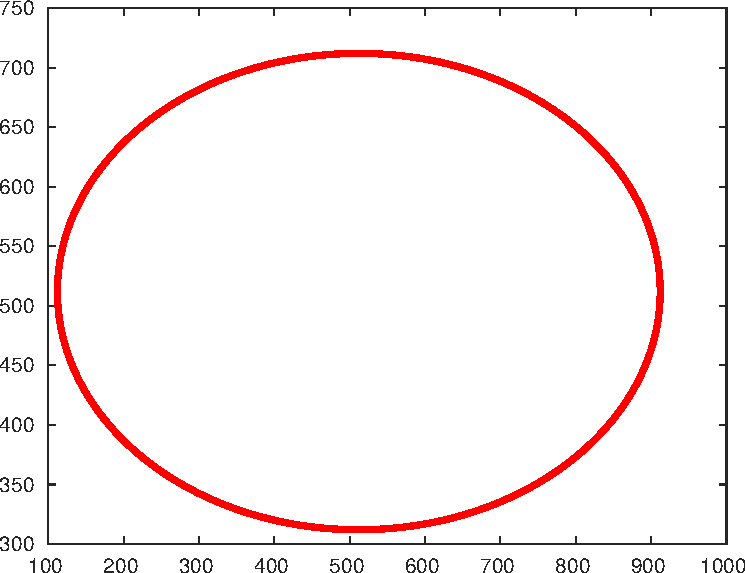
\includegraphics[width=.45\linewidth]{ellipse.pdf}
 \caption{Initialization of the active contour.}
 \label{fig:active_contours:matlab:ellipse}
\end{figure}


The different parameters are defined by:
\begin{matlab}
alpha = .00001;
beta  = .05;
gamma = 200;
iterations = 1000;
\end{matlab}

\subsection{Matrix construction}
This is maybe the hardest part of this code, with the use of the \minline{spdiags} function.
\begin{matlab}
N = length(x);
X = [-beta alpha+4*beta -2*alpha-6*beta alpha+4*beta -beta -beta alpha+4*beta -beta alpha+4*beta];
B = repmat(X, N, 1);
A = full(spdiags(B, [-2 -1 0 1 2 N-2 N-1 -N+2 -N+1], N, N));
AA = eye(N) - gamma*A;
\end{matlab}

Be aware that in \matlabregistered{}, for efficiency reasons, the invert of the matrix can be written as \minline{inv(A)*y=A\ y}.

\subsection{External forces}
\begin{matlab}
% define convolution kernels
hgauss = fspecial('gaussian', 100, 30);
hprewitt  = fspecial('prewitt');

% gaussian filter
G = imfilter(I, hgauss, 'replicate');
% gradient (prewitt) and its norm
Fy= imfilter(G, hprewitt, 'symmetric');
Fx= imfilter(G, hprewitt', 'symmetric');
G = sqrt(Fx.^2+Fy.^2);

% orientation of previous gradient
Fy= imfilter(-G, hprewitt, 'symmetric');
Fx= imfilter(-G, hprewitt', 'symmetric');
\end{matlab}

\subsection{Display results}
To enhance the role of the external forces, the arrows showing the force are displayed (\minline{quiver} function).

\begin{matlab}
imshow(I,[])
hold on
plot([x;x(1)], [y; y(1)], 'g', 'linewidth', 3);

%% display arrows for external forces
step=20;
subx = 1:step:size(I,1);
suby = 1:step:size(I,2);
[Xa, Ya] = meshgrid(subx, suby);
quiver(Xa, Ya, Fx(subx, suby), Fy(subx,suby));
\end{matlab}

\subsection{Convergence algorithm}
\begin{matlab}
h = waitbar(0, 'snake converging...');
% iterations
for index = 1:iterations,
    % interpolate values of forces
    fex = interp2(Fx, x, y, 'linear');
    fey = interp2(Fy, x, y);
    
    x = AA\(x+gamma*fex);
    y = AA\(y+gamma*fey);
    % display
    if mod(index,10)==0
        plot([x;x(1)], [y;y(1)], 'b');
    end
    waitbar(index/iterations);
end
plot([x;x(1)], [y;y(1)], 'r', 'linewidth', 3);
close(h)

\end{matlab}

The results are displayed in Fig.\ref{fig:active_contours:matlab:result}.

\begin{figure}
 \centering
 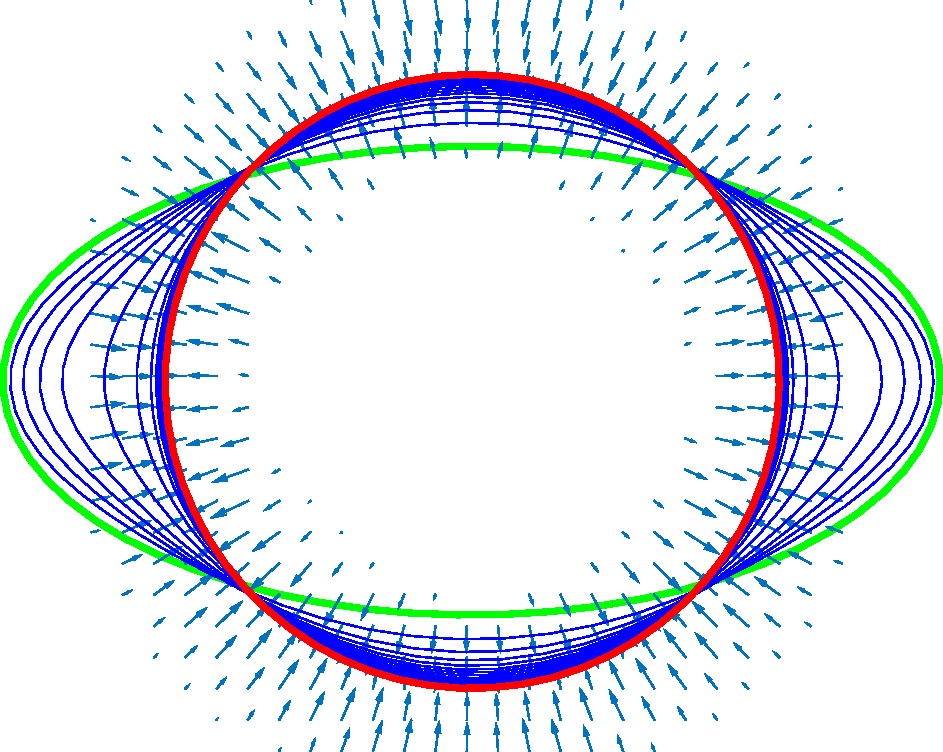
\includegraphics[width=10cm]{convergence.pdf}
 \caption{Result of the snake converging toward the disk, after 1000 iterations with the proposed parameters. 
 The green ellipse is the original snake, the red snake shows the final result. Blue snakes are intermediate results.}
 \label{fig:active_contours:matlab:result}
\end{figure}
